\documentclass[
11pt, % Set the default font size, options include: 8pt, 9pt, 10pt, 11pt, 12pt, 14pt, 17pt, 20pt
%t, % Uncomment to vertically align all slide content to the top of the slide, rather than the default centered
%aspectratio=169, % Uncomment to set the aspect ratio to a 16:9 ratio which matches the aspect ratio of 1080p and 4K screens and projectors
]{beamer}

\graphicspath{{Images/}{./}} % Specifies where to look for included images (trailing slash required)

\usepackage{todonotes}
\usepackage{graphicx}
\usepackage{xcolor}
\usepackage{subfig}
%%\usepackage[noend]{algpseudocode}


\usepackage{algorithm}
\usepackage{algorithmic}

\usepackage{blkarray}
\usepackage{amsmath}
\usepackage{xspace}
\usepackage{float}


\usepackage{tikz}
\usetikzlibrary{matrix, decorations, patterns, positioning, shapes, calc, intersections, arrows, fit}

\usetikzlibrary{patterns}
\usetikzlibrary{fit,calc,positioning,decorations.pathreplacing,matrix,3d, hobby}

\usepackage{booktabs} % Allows the use of \toprule, \midrule and \bottomrule for better rules in tables


\newcommand{\brown}[1]{{\color{brown} #1 }}

%% Colors from https://latexcolor.com/
\definecolor{pastelviolet}{rgb}{0.8, 0.6, 0.79}
\definecolor{babyblueeyes}{rgb}{0.63, 0.79, 0.95}
\definecolor{pastelyellow}{rgb}{0.99, 0.99, 0.59}
\definecolor{pastelgreen}{rgb}{0.47, 0.87, 0.47}
\definecolor{pastelred}{rgb}{1.0, 0.41, 0.38}
\colorlet{patternblue}{blue!60}


\colorlet{darkred}{red!80!black}
\colorlet{darkblue}{blue!80!black}
\newcommand<>{\darkred}[1]{{\color{darkred}{#1}}}
\newcommand<>{\darkblue}[1]{{\color#2{blue!50!black!100}{#1}}}

\newcommand{\A}{\mathbf{A}}
\newcommand{\B}{\mathbf{B}}
\newcommand{\CC}{\mathbf{C}}

\usetheme{Madrid}





%----------------------------------------------------------------------------------------
%	PRESENTATION INFORMATION
%----------------------------------------------------------------------------------------

\title[Matrix multiplication]{Communication costs of parallel matrix multiplications} % The short title in the optional parameter appears at the bottom of every slide, the full title in the main parameter is only on the title page

%\subtitle{Optional Subtitle} % Presentation subtitle, remove this command if a subtitle isn't required

\author[Suraj Kumar]{Suraj Kumar} % Presenter name(s), the optional parameter can contain a shortened version to appear on the bottom of every slide, while the main parameter will appear on the title slide

\institute[Inria \& ENS Lyon]{Inria \& ENS Lyon \\ \smallskip Email:\textit{suraj.kumar@inria.fr}} % Your institution, the optional parameter can be used for the institution shorthand and will appear on the bottom of every slide after author names, while the required parameter is used on the title slide and can include your email address or additional information on separate lines

\date[CR12]{CR12: September 2023\\ \smallskip\small https://surakuma.github.io/courses/daamtc.html} % Presentation date or conference/meeting name, the optional parameter can contain a shortened version to appear on the bottom of every slide, while the required parameter value is output to the title slide

%----------------------------------------------------------------------------------------

\begin{document}
	
	%----------------------------------------------------------------------------------------
	%	TITLE SLIDE
	%----------------------------------------------------------------------------------------
	
	\begin{frame}
		\titlepage % Output the title slide, automatically created using the text entered in the PRESENTATION INFORMATION block above
	\end{frame}
	\section{2D-algorithms}
	\begin{frame}{Table of Contents}		
		\tableofcontents[currentsection,hideallsubsections] % Output the table of contents (all sections on one slide)		
	\end{frame}
	\begin{frame}{Matrix multiplication with 2D layout}
		\begin{itemize}
			\item Consider processors are arranged in a 2-dimensional grid
			\item Processors can broadcast along rows and columns
		\end{itemize}
	\begin{center}
		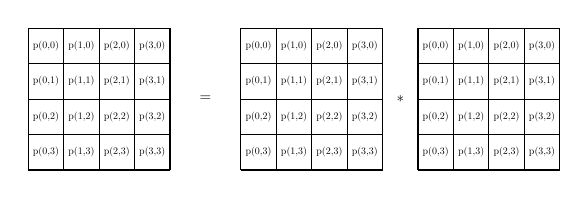
\begin{tikzpicture}[scale=0.45, every node/.style={transform shape}]
		\def\xstep{0}
		\foreach \x in {0,1,2,3, 4}
		{
			\draw (\xstep,\x) -- (\xstep+4,\x);
			\draw (\xstep+\x,0) -- (\xstep+\x,4);
		}
		\foreach \x in {0,1,2,3}
			\foreach \y in {0,1,2,3}
			\node [scale=0.8] at (\xstep+ \x+0.5 , 3.5-\y) {p(\x,\y)};
			
		\node [scale=1.2] at (5,2) {$=$};
		
		\def\xstep{6}
		\foreach \x in {0,1,2,3, 4}
		{
			\draw (\xstep,\x) -- (\xstep+4,\x);
			\draw (\xstep+\x,0) -- (\xstep+\x,4);
		}
		\foreach \x in {0,1,2,3}
		\foreach \y in {0,1,2,3}
		\node [scale=0.8] at (\xstep+ \x+0.5 , 3.5-\y) {p(\x,\y)};
		\node [scale=1.2] at (10.5,2) {$*$};
		\def\xstep{11}
		\foreach \x in {0,1,2,3, 4}
		{
			\draw (\xstep,\x) -- (\xstep+4,\x);
			\draw (\xstep+\x,0) -- (\xstep+\x,4);
		}
		\foreach \x in {0,1,2,3}
		\foreach \y in {0,1,2,3}
		\node [scale=0.8] at (\xstep+ \x+0.5 , 3.5-\y) {p(\x,\y)};
		\end{tikzpicture}
	\end{center}
	\end{frame}
	\section{Communication lower bounds}
	\begin{frame}{Table of Contents}		
		\tableofcontents[currentsection,hideallsubsections] % Output the table of contents (all sections on one slide)		
	\end{frame}
	\begin{frame}{Notations \& Settings}
		\begin{itemize}
			\item $C=AB$, where $A \in \mathbb{R}^{n_1\times n_2}, B \in \mathbb{R}^{n_2\times n_3}$, and $C \in \mathbb{R}^{n_1\times n_3}$
			\item Let $d_1=\min(n_1,n_2,n_3) \le d_2=median(n_1,n_2,n_3) \le d_3 = \max(n_1,n_2,n_3)$
		\end{itemize}
	\vfill			
				\begin{block}{Settings}
					\begin{itemize}
						\item $P$ number of processors
						\item The algorithm load balances the computations
						\item One copy of data is in the system
						\begin{itemize}
							\item There exists a processor whose input data at the start plus output data at the end  must be at most $\frac{d_1d_2+d_1d_3+d_2d_3}{P}$ words -- will analyze data transfers for this processor   
						\end{itemize}
						\item Focus on bandwidth cost (volume of data transfers)
					\end{itemize}
				\end{block}	


	\end{frame}
	\begin{frame}{Constraints for Matrix Multiplications}
					\begin{itemize}
			\item Loomis-Whitney inequalitiy: for $d-1$ dimensional projections
			\begin{itemize}
				\item For the $2$d object $G$, $ Area(G) \le \phi_x \phi_y$
				\item For the $3$d object $H$, $Volume(H) \le \sqrt{\phi_{xy}\phi_{yz}\phi_{xz}}$
				%%		\item $2$-dimensional object $A$ and its $1$-dimensional projections are $\phi_x$ and $\phi_y$, then $\phi_x \phi_y \ge Area(A)$
				%%		\item $3$-dimensional object $B$ and its $2$-dimensional projections are $\phi_{xy}$, $\phi_{yz}$ and $\phi_{xz}$, then $(\phi_{xy}\phi_{yz}\phi_{xz})^\frac{1}{2} \ge Volume(B)$
			\end{itemize}
		\end{itemize}
		
		\begin{center}
			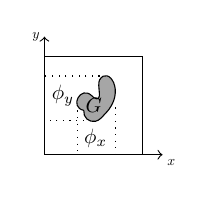
\begin{tikzpicture}[scale=0.25, every node/.style={transform shape}]
			\draw (0,0) -- ++(5,0) -- ++(0, 5) -- ++(-5,0) -- cycle;
			\draw [<->] (0,6) -- (0,0) -- (6,0);
			\node [below right, scale=2] at (6,0) {$x$};
			\node [left, scale=2] at (0,6) {$y$};
			
			\draw [fill=gray!70] (2,2.25) to [curve through={(2.4,3) .. (2.5,2.9) .. (2.8,3.8) .. (3.1,2.1) .. (2.6,1.7)}] (2,2.25);
			
			\node [scale=3] at (2.5,2.5) {$G$};
			\draw [dotted] (1.7,2.25) -- (1.7,0);
			\draw [dotted] (3.6,2.4) -- (3.6,0);
			
			\node[above, scale=3] at (2.6,0) {$\phi_x$};
			
			\draw [dotted] (2,1.75) -- (0,1.75);
			\draw [dotted] (2.8,4) -- (0,4);
			
			\node[right, scale=3] at (0,3) {$\phi_y$};
			\end{tikzpicture}
			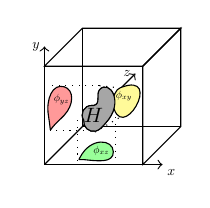
\begin{tikzpicture}[scale=0.25, every node/.style={transform shape}]
			\draw (0,0) -- ++(5,0) -- ++(0, 5) -- ++(-5,0) -- cycle;
			\draw (0,5,0) -- ++(0,0, -5) -- ++(5,0,0) -- ++(0,0,5) -- cycle;
			\draw (5,0,0) -- ++(0,0,-5) -- ++(0,5,0) -- ++(0,0,5) -- cycle;
			\draw (0,0,-5) -- ++(5,0,0) -- ++(0,5,0) -- ++(-5,0,0) -- cycle;
			\draw [<->] (0,6) -- (0,0) -- (6,0);
			\draw [->] (0,0,0) -- (0,0,-12);
			\node [left, scale=2, rotate=0] at (0,0,-12) {$z$};
			\node [below right, scale=2] at (6,0) {$x$};
			\node [left, scale=2] at (0,6) {$y$};
			
			\draw [fill=gray!70] (2,2.25) to [curve through={(2.4,3) .. (2.5,3) .. (2.8,3.8) .. (3.1,2.1) .. (2.6,1.7)}] (2,2.25);
			
			%				\node [scale=2] at (2.5,2.5) {$G$};
			\draw [dotted] (1.7,2.25) -- (1.7,0.2);
			\draw [dotted] (3.6,2.4) -- (3.6,0.3);
			
			\draw [fill=green!40] (1.75,0.25) to [curve through={(1.8, 0.35) .. (3.5, 0.65) .. (2,0.25)}] (1.75,0.25);
			\node[above, scale=1.5] at (2.6,0,-0.75) {$\phi_{xz}$};
			
			\draw [dotted] (2,1.75) -- (0.3,1.75);
			\draw [dotted] (2.8,4) -- (0.385,4);
			
			\draw [fill=red!40] (0.3, 1.75) to [curve through={(0.5,2) .. (1, 2.5) .. (1,3.95) .. (0.2, 2.5)}] (0.3,1.75);
			\node[right, scale=1.5] at (0,3, -0.75) {$\phi_{yz}$};
			
			\draw [fill=yellow!40] (3.85,3.9) to [curve through={(3.7,3.8) .. (3.5,3.4) .. (3.45,3.2)}] (3.85, 3.9);
			\node [scale=1.5] at (3.65,3.1,-1) {$\phi_{xy}$};
			\draw [dotted] (2.8,4) -- (3.8,3.9);
			\draw [dotted] (2.56,1.65) -- (4,2.5);
			
			\draw [fill=gray!70] (2,2.25) to [curve through={(2.4,3) .. (2.5,3) .. (2.8,3.8) .. (3.1,2.1) .. (2.6,1.7)}] (2,2.25);
			
			\node [scale=3] at (2.5,2.5) {$H$};
			\end{tikzpicture}
		\end{center}
	\vspace*{-0.7cm}
		\begin{center}
			\begin{align*}
			&\text{for $i = 1{:}n_1$, for $k = 1{:}n_2$, for $j = 1{:}n_3$}\\
			&\quad \quad C[i][j] += A[i][k]*B[k][j]
			\end{align*}
		\end{center}
		\begin{itemize}
			\item Total number of multiplications = $n_1n_2n_3$
			\item A processor performs $\frac{n_1n_2n_3}{P}$ amount of multiplications
			\item Optimization problem: 
			\begin{align*}
			Minimize &\ \phi_A + \phi_B + \phi_C \  \text{ s.t.}\\
			\phi_A^\frac{1}{2} \phi_B^\frac{1}{2}  \phi_C^\frac{1}{2} & \ge \frac{n_1n_2n_3}{P}
			\end{align*}
		\end{itemize}

	\end{frame}
	\begin{frame}{Extra constraints}
		
	\begin{center}
		\begin{align*}
		&\text{for $i = 1{:}n_1$, for $k = 1{:}n_2$, for $j = 1{:}n_3$}\\
		&\quad \quad C[i][j] += A[i][k]*B[k][j]
		\end{align*}
	\end{center}
	
	\begin{itemize}
		\item Each element of $A$ (resp. $B$) is involved in $n_3$ (resp. $n_1$) multiplications
		\begin{itemize}
			\item To perform at least $\frac{n_1n_2n_3}{P}$ multiplications: $\phi_A \ge \frac{n_1n_2}{P}, \phi_B \ge \frac{n_2n_3}{P}$
		\end{itemize}
		\item Each element of $C$ is the sum of $n_2$ multiplications, therefore $\phi_C \ge \frac{n_1n_3}{P}$
		\item Projections can be at max the size of the arrays: $\phi_A \le n_1n_2$, $\phi_B \le n_2n_3$, $\phi_C \le n_1n_3$ 
	\end{itemize}

	\end{frame}

\begin{frame}{Optimization problem for communication lower bounds}
	
	{\small$\bullet$ Projections ($\phi_A,  \phi_B, \phi_C$) indicate the amount of array accesses\\
		$\bullet$ Communication lower bound = $\phi_A + \phi_B + \phi_C - \text{data owned by the processor}$
		\begin{minipage}{0.45\linewidth}
			\begin{center}
				\begin{align*}
				Minimize &\ \phi_A + \phi_B + \phi_C \  \text{ s.t.}\\
				\phi_A^\frac{1}{2} \phi_B^\frac{1}{2}  \phi_C^\frac{1}{2} & \ge \frac{n_1n_2n_3}{P}\\
				\frac{n_1n_2}{P} \le &\phi_A \le n_1n_2\\
				\frac{n_2n_3}{P} \le &\phi_B \le n_2n_3\\
				\frac{n_1n_3}{P} \le &\phi_C \le n_1n_3
				\end{align*}
			\end{center}
		\end{minipage}
		\begin{minipage}{0.5\linewidth}
			\vspace*{-0.15cm}\begin{block}{Generalized version (in terms of $d_1$, $d_2$, $d_3$)}
				\vspace*{-0.35cm}\begin{align*}
				Minimize &\ \phi_1 + \phi_2 + \phi_3 \  \text{ s.t.}\\
				\phi_1^\frac{1}{2} \phi_2^\frac{1}{2}  \phi_3^\frac{1}{2} & \ge \frac{d_1d_2d_3}{P}\\
				\frac{d_1d_2}{P} \le &\phi_1 \le d_1d_2\\
				\frac{d_1d_3}{P} \le &\phi_2 \le d_1d_3\\
				\frac{d_2d_3}{P} \le &\phi_3 \le d_2d_3\\
				d_1 \le & d_2 \le d_3
				\end{align*}
			\end{block}
		\end{minipage}
		
		
}\end{frame}
\begin{frame}{Amount of accesses and communication lower bounds}
	$\bullet$ Estimate the solution based on Lagrange multipliers\\
	$\bullet$ Prove optimality using all Karush–Kuhn–Tucker (KKT) conditions are satisfied
	\begin{block}{\small Amount of accesses =$\phi_1 + \phi_2 + \phi_3$}
		\begin{center}
			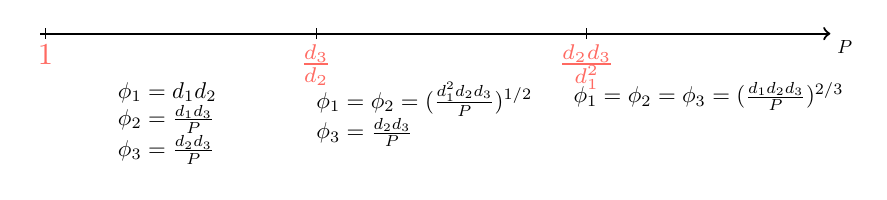
\begin{tikzpicture}[scale=0.6875, every node/.style={transform shape}]
			%%\draw (-2,0) -- node[below] {a} ++(2,0) -- node[above] {b} ++(2,0);
			%%\draw (-0.1,0) -- ++(5,0) -- ++(5,0);
			\draw [->, thick] (-0.1,0) -- (14.5,0) node [below right] {$P$};
			\draw (0, 0.1) -- node [below, pastelred, scale=1.6]{$1$}(0,-0.1);
			\draw (5, 0.1) -- node [below, pastelred, scale=1.6]{$\frac{d_3}{d_2}$}(5,-0.1);
			\draw (10, 0.1) -- node [below, pastelred, scale=1.6] {$\frac{d_2d_3}{d_1^2}$}(10,-0.1);
			
			\node[align=left,below,scale=1.2] at (2.25, -0.75) {$\phi_1 = d_1d_2$\\ $\phi_2=\frac{d_1d_3}{P}$\\ $\phi_3 = \frac{d_2d_3}{P}$};
			\node[align=left,below,scale=1.2] at (7, -0.75) {$\phi_1 =\phi_2= (\frac{d_1^2d_2d_3}{P})^{1/2}$\\ $\phi_3 = \frac{d_2d_3}{P}$};
			\node[align=center,below,scale=1.2] at (12.25, -0.75) {$\phi_1 = \phi_2 = \phi_3 = (\frac{d_1d_2d_3}{P})^{2/3}$};	
			\end{tikzpicture}
		\end{center} 
	\end{block}
	\begin{block}{\small Communication Lower Bounds (Amount of Data Transfers)}
		\begin{center}
			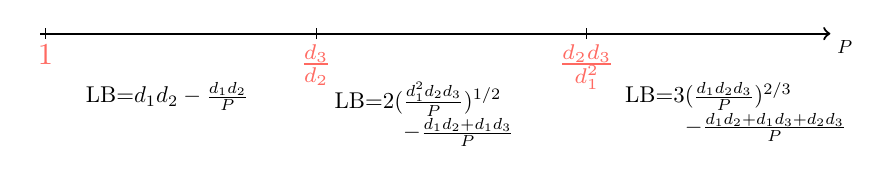
\begin{tikzpicture}[scale=0.6875, every node/.style={transform shape}]
			%%\draw (-2,0) -- node[below] {a} ++(2,0) -- node[above] {b} ++(2,0);
			%%\draw (-0.1,0) -- ++(5,0) -- ++(5,0);
			\draw [->, thick] (-0.1,0) -- (14.5,0) node [below right] {$P$};
			\draw (0, 0.1) -- node [below, pastelred, scale=1.6]{$1$}(0,-0.1);
			\draw (5, 0.1) -- node [below, pastelred, scale=1.6]{$\frac{d_3}{d_2}$}(5,-0.1);
			\draw (10, 0.1) -- node [below, pastelred, scale=1.6] {$\frac{d_2d_3}{d_1^2}$}(10,-0.1);
			
			\node[align=left,below,scale=1.2] at (2.25, -0.75) {LB=$d_1d_2 -\frac{d_1d_2}{P}$};
			\node[align=left,below,scale=1.2] at (7, -0.75) {LB=$2(\frac{d_1^2d_2d_3}{P})^{1/2}$\\
				$\qquad\quad-\frac{d_1d_2+d_1d_3}{P}$};
			\node[align=center,below,scale=1.2] at (12.25, -0.75) {LB=$3(\frac{d_1d_2d_3}{P})^{2/3}$\\ $\qquad\qquad\quad -\frac{d_1d_2+d_1d_3+d_2d_3}{P}$};	
			\end{tikzpicture}
		\end{center}
	\end{block}
\end{frame}
	\section{Parallel algorithms}
	\begin{frame}{Table of Contents}		
	\tableofcontents[currentsection,hideallsubsections] % Output the table of contents (all sections on one slide)		
	\end{frame}
\begin{frame}{Design of communication optimal algorithms for $C=AB$}
	
	\begin{exampleblock}{\small Arrangements of $8$ processors}
		\begin{center}
			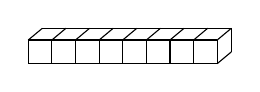
\begin{tikzpicture}[scale=0.3, every node/.style={transform shape}]	
			\foreach \x in {0, 1, 2, 3, 4, 5, 6, 7, 8}
			\draw (-\x, 0) -- (-\x, 1);
			
			\foreach \x in {0, 1, 2, 3, 4, 5, 6, 7, 8}
			\draw (-\x, 1) -- (-\x+0.6, 1.5);
			
			\draw (-8,0) -- (0,0);
			\draw (-8,1) -- (0,1);
			\draw (-8+0.6,1+0.5) -- (0+0.6,1+0.5);
			
			\draw (0,0) -- (0.6,0.5);
			\draw (0.6,0.5) -- (0.6,1.5);
			\end{tikzpicture}$\qquad$
			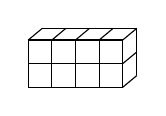
\begin{tikzpicture}[scale=0.3, every node/.style={transform shape}]	
			\foreach \x in {0, 1, 2, 3, 4}
			\draw (-\x, 0) -- (-\x, 1);
			
			\foreach \x in {0, 1, 2, 3, 4}
			\draw (-\x, 0) -- (-\x, -1);
			
			\foreach \x in {0, 1, 2, 3, 4}
			\draw (-\x, 1) -- (-\x+0.6, 1.5);
			
			\draw (-4,0) -- (0,0);
			\draw (-4,-1) -- (0,-1);
			\draw (-4,1) -- (0,1);
			\draw (-4+0.6,1+0.5) -- (0+0.6,1+0.5);
			
			\draw (0,0) -- (0.6,0.5);
			\draw (0.6,0.5) -- (0.6,1.5);
			
			\draw (0,-1) -- (0.6,-1+0.5);
			\draw (0.6,-1+0.5) -- (0.6,0.5);
			\end{tikzpicture}$\qquad$
			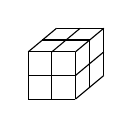
\begin{tikzpicture}[scale=0.3, every node/.style={transform shape}]
			
			\def\xref{0.6}
			\def\yref{0.5}
			
			\foreach \x in {0, 1, 2}
			\draw (-2, \x) -- (0, \x);
			
			\foreach \x in {0, 1, 2}
			\draw (0, \x)--(2*\xref, 2*\yref+\x);
			
			\draw (0,0) -- (0,2);
			\draw (-1,0) -- (-1,2);
			\draw (-2,0)--(-2,2);
			\draw (\xref,\yref) -- (\xref, 2+\yref);
			\draw (2*\xref,2*\yref) -- (2*\xref, 2+ 2*\yref);
			
			\draw (-2,2) -- (-2+2*\xref, 2+2*\yref);
			\draw (-1,2) -- (-1+2*\xref, 2+2*\yref);
			
			\draw (-2+2*\xref, 2+2*\yref) -- (2*\xref, 2+2*\yref);
			\draw (-2+\xref, 2+\yref) -- (\xref, 2+\yref);
			\end{tikzpicture}
		\end{center}
	\end{exampleblock}
	\vfill
	\begin{minipage}{0.585\linewidth}{\small	
			\begin{itemize}
				\item $P$ is organized into $p_1 \times p_2 \times p_3$ logical grid
				\item Select $p_1,p_2$ and $p_3$ based on the communication lower bounds
				\item Gather $A$ on the set of processors along each slice of $p_3$
				\item Gather $B$ on the set of processors along each slice of $p_1$
				\item Perform local computation
				\item Perform reduce operation along $p_2$ to obtain $C$ 
			\end{itemize}
	}\end{minipage}
	\begin{minipage}{0.4\linewidth}
		\begin{center}
			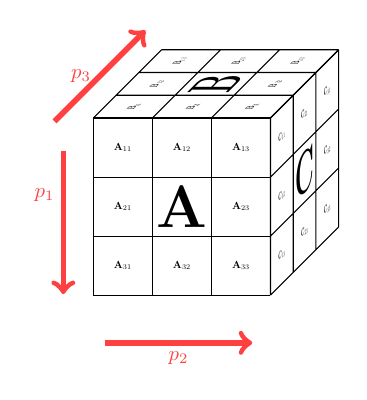
\begin{tikzpicture}[every node/.append style={transform shape},scale=0.75]
			% draw lines signifying collectives
			%%		\draw[line width=2,->,red!75] (-2.5,-1.5,0) -- (0,-1.5,0) node [right] {$p_2$};
			\draw[line width=2,->,red!75] (-2.5,-1.5,0) -- (-1.25,-1.5,0) node [below] {$p_2$} -- (0,-1.5,0);
			\draw[line width=2,->,red!75] (-3.2,1.75,0) -- (-3.2,1,0) node [left] {$p_1$} -- (-3.2,-0.675,0);
			\draw[line width=2,->,red!75] (-3.35,2.25,0) -- (-3.35,2.25,-2) node [left] {$p_3$} -- (-3.35,2.25,-4);
			%%		\draw[line width=3,stealth-stealth,red!75] (0,2,0) -- (-2.25,2,0);
			%%		\draw[line width=3,stealth-stealth,red!75] (0,2,0) -- (0,-.25,0);
			% right face of comp cube
			\begin{scope}[canvas is yz plane at x=.5,rotate=-90,yscale=-1,shift={(-.5,-3+.5)}]
			%%\draw[fill=red!25] (0,0) rectangle (1,1);
			%%\draw[fill=red!75] (2/3,0) rectangle (1,1);
			\draw[black] (0,0) grid (3,3);
			%%\draw[black,xscale=1/3,dotted] (0,0) grid (3,1);
			\node[yscale=-1,scale=2] at (3/2,3/2) {\Large $\CC$};
			\node[yscale=-1,scale=.5] at (1/2,1/2) {$\CC_{11}$};
			\node[yscale=-1,scale=.5] at (1/2,3/2) {$\CC_{12}$};
			\node[yscale=-1,scale=.5] at (1/2,5/2) {$\CC_{13}$};
			\node[yscale=-1,scale=.5] at (3/2,1/2) {$\CC_{21}$};
			\node[yscale=-1,scale=.5] at (3/2,5/2) {$\CC_{23}$};
			\node[yscale=-1,scale=.5] at (5/2,1/2) {$\CC_{31}$};
			\node[yscale=-1,scale=.5] at (5/2,3/2) {$\CC_{32}$};
			\node[yscale=-1,scale=.5] at (5/2,5/2) {$\CC_{33}$};
			\end{scope}
			% front face of comp cube
			\begin{scope}[canvas is yx plane at z=.5,yscale=-1,rotate=180,shift={(-3+.5,-3+.5)}]
			%%\draw[fill=red!25] (0,2) rectangle (1,3);
			%%\draw[fill=red!75] (0,2) rectangle (1,7/3);
			\draw[black] (0,0) grid (3,3);
			%%\draw[black,shift={(0,2)},yscale=1/3,dotted] (0,0) grid (1,3);
			\node[rotate=90,scale=2] at (3/2,3/2) {\Large $\A$};
			\node[rotate=90,scale=.5] at (1/2,1/2) {$\A_{11}$};
			\node[rotate=90,scale=.5] at (1/2,3/2) {$\A_{12}$};
			\node[rotate=90,scale=.5] at (1/2,5/2) {$\A_{13}$};
			\node[rotate=90,scale=.5] at (3/2,1/2) {$\A_{21}$};
			\node[rotate=90,scale=.5] at (3/2,5/2) {$\A_{23}$};
			\node[rotate=90,scale=.5] at (5/2,1/2) {$\A_{31}$};
			\node[rotate=90,scale=.5] at (5/2,3/2) {$\A_{32}$};
			\node[rotate=90,scale=.5] at (5/2,5/2) {$\A_{33}$};
			\end{scope}
			% top face of comp cube
			\begin{scope}[canvas is zx plane at y=(3-.5),rotate=90,shift={(-3+.5,-.5)}]
			%%\draw[fill=red!25] (2,0) rectangle (3,1);
			%%\draw[fill=red!75] (2,0) rectangle (3,1/3);
			\draw[black] (0,0) grid (3,3);
			%%\draw[black,shift={(2,0)},yscale=1/3,dotted] (0,0) grid (1,3);
			\node[rotate=90,scale=2] at (3/2,3/2) {\Large $\B$};
			\node[rotate=90,scale=.5] at (1/2,1/2) {$\B_{11}$};
			\node[rotate=90,scale=.5] at (1/2,3/2) {$\B_{12}$};
			\node[rotate=90,scale=.5] at (1/2,5/2) {$\B_{13}$};
			\node[rotate=90,scale=.5] at (3/2,1/2) {$\B_{21}$};
			\node[rotate=90,scale=.5] at (3/2,5/2) {$\B_{23}$};
			\node[rotate=90,scale=.5] at (5/2,1/2) {$\B_{31}$};
			\node[rotate=90,scale=.5] at (5/2,3/2) {$\B_{32}$};
			\node[rotate=90,scale=.5] at (5/2,5/2) {$\B_{33}$};
			\end{scope}
			\end{tikzpicture}
		\end{center}
	\end{minipage}
\end{frame}

\begin{frame}{Communication optimal algorithms}
	\vspace*{-0.25cm}\begin{block}{\small Data Distribution ($P$ is organized into a $p_1 \times p_2 \times p_3$ grid)}
		\begin{minipage}{0.75\linewidth}{\small	
				\begin{itemize}
%					\item Select $p_1,p_2$, and $p_3$ based on communication lower bounds
					\item Each processor has $\frac{1}{P}$th amount of input and output variables
					\item $A_{31} = A(2\frac{n_1}{p_1}+1:3\frac{n_1}{p_1}, 1:\frac{n_2}{p_2})$ is evenly distributed among $(3,1, *)$ processors
					\item $B_{12} =  B(1:\frac{n_2}{p_2}, \frac{n_3}{p_3}+1:2\frac{n_3}{p_3})$ is evenly distributed among $(*,1,2)$ processors  
				\end{itemize}
		}\end{minipage}
		\begin{minipage}{0.2\linewidth}
			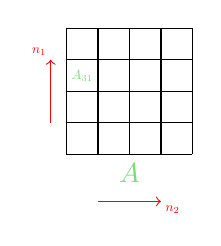
\begin{tikzpicture}[scale=0.4, every node/.style={transform shape}]
			\def\xref{0.6}
			\def\yref{0.5}
			
			\foreach \y in {0, 1, 2, 3, 4}
			\draw (-2, \y) -- (2, \y);
			
			\foreach \x in {-2, -1, 0, 1, 2}
			\draw (\x, 0) -- (\x, 4);
			
			\node [below, pastelgreen, scale=2.5] at (0,0) {$A$};
			
			
			\node [ pastelgreen, scale=1.2] at (-1.5,2.5) {$A_{31}$};
			
			\draw [->, red] (-1,-1.5) -- (1,-1.5) node [below right, scale=1.2] {$n_2$};
			\draw [->, red] (-2.5,1) -- (-2.5,3) node [ above left, scale=1.2] {$n_1$};
			\end{tikzpicture}
		\end{minipage}
	\end{block}
	
	\vspace*{-0.3cm}\begin{algorithm}[H]{\footnotesize
			\caption{$C=AB$ Matrix Multiplication Algorithm}
			\begin{algorithmic}[1]
				\STATE $(p_1^\prime, p_2^\prime, p_3^\prime)$ is my processor id
				\STATE //All-gather input matrices $A$ and $B$
				\STATE $A_{p_1^\prime p_2^\prime}$ = All-Gather($A$, $(p_1^\prime, p_2^\prime, *)$)
				\STATE $B_{p_2^\prime p_3^\prime}$ = All-Gather($B$, $(*, p_2^\prime, p_3^\prime)$)
				%%			\STATE //Perform local Matrix Multiplication in a temporary variable $T$
				\STATE $T$ = Local-Matrix-Multiplication($A_{p_1^\prime p_2^\prime}, B_{p_2^\prime p_3^\prime} $) // Local matrix multiplication in a temporary
				%%			\STATE //Reduce-scatter the output matrix in $C_{p_1^\prime p_3^\prime}$
				\STATE Reduce-Scatter($C_{p_1^\prime p_3^\prime}$, T,  $(p_1^\prime,*,p_3^\prime)$) // Reduce-scatter the output
			\end{algorithmic}
	}\end{algorithm}
\end{frame}
\begin{frame}{Cost Analysis and Open Questions}
	\begin{block}{Cost Analysis}
		\begin{itemize}
			\item Total amount of multiplications per processor = $\frac{n_1n_2n_3}{p_1p_2p_3} = \frac{n_1n_2n_3}{P}$
			%%		\item Amount of data transfers to perform All-Gather/Reduce-Scatter operation on $Q$ processors = $(1-\frac{1}{Q})w$, $w$ is amount of total data after All-Gather or before Reduce-Scatter operation
			\item Total data transfers = $\frac{n_1n_2}{p_1p_2} + \frac{n_2n_3}{p_2p_3} + \frac{n_1n_3}{p_1p_3} - \frac{n_1n_2+n_2n_3+n_1n_3}{P}$   
		\end{itemize}
	\end{block}
	\vfill
	\begin{block}{Open Questions}
		\begin{itemize}
%			\item How to select $p_1, p_2, p_3$?
			\item Are communication lower bounds achievable for all matrix dimensions?
		\end{itemize}
	\end{block}
	
\end{frame}


\end{document} 